\begin{frame}{stateful firewall}
    \begin{itemize}
    \item common policy: allow outgoing connections only
    \vspace{.5cm}
    \item prior approach:
        \begin{itemize}
        \item drop incoming non-TCP, or TCP SYN
        \end{itemize}
    \item problems:
        \begin{itemize}
        \item disallowing UDP-based protocols (example: DNS over UDP, HTTP/3)
        \item disallowing normal ICMP (example: ICMP ping replies)
        \item allowing unsolicited TCP packets
        \end{itemize}
    \end{itemize}
\end{frame}

\begin{frame}{keeping state}
    \begin{itemize}
    \item outgoing connections only?
    \item really want to track list of \textit{connections}
    \vspace{.5cm}
    \item most common form of \textit{stateful firewall}
    \end{itemize}
\end{frame}

\begin{frame}{Linux conntrack}
    \begin{itemize}
    \item in-kernel table of active ``connections''
    \item includes notion of connections for UDP, ICMP, etc.
        \begin{itemize}
        \item heuristic guesses since protocol has no connect/close operation
        \end{itemize}
    \item maintains table of (proto, source host+port, dest host+port)
    \item packets marked with connection state
        \begin{itemize}
        \item new, established, \myemph<2>{related}, invalid
        \end{itemize}
    \end{itemize}
\end{frame}

\begin{frame}{related connection example}
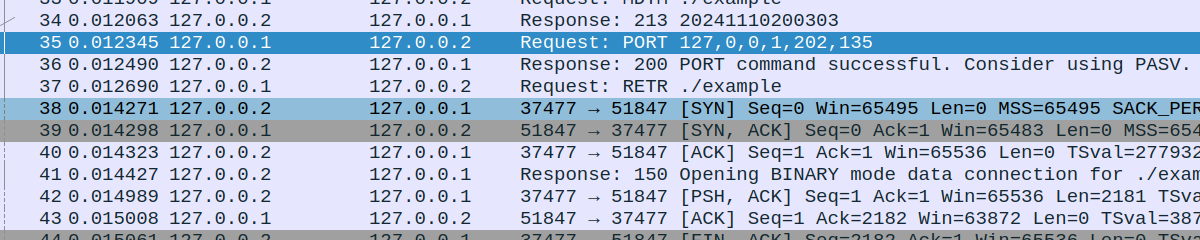
\includegraphics[width=\textwidth]{../fire/ftp-port-ex.png}
\begin{itemize}
\item FTP --- uses separate control + data TCP connections
\item can be client or server created connections:
\vspace{.5cm}
\item PORT command: server creates data connection to specified address
    \begin{itemize}
    \item problem for firewalls: looks like `fresh' TCP connection
    \end{itemize}
\item PASV command: server gets address for client to conect
    \begin{itemize}
    \item most FTP clients default to this mode
    \end{itemize}
\item in theory, allows direct server-to-server transfers
    \begin{itemize}
    \item one client uses PASV on one server, PORT on the other
    \end{itemize}
\end{itemize}
\end{frame}

\begin{frame}{Linux conntrack timeouts}
    \begin{itemize}
    \item problem: TCP connection with no activity for 30 minutes
    \item should it stay in table?
    \item how about after 8 hours?
    \end{itemize}
\end{frame}
